\section{Experimental Study}\label{sec:expr}
We implemented our approach in a tool called \tool written in C++ interfacing Minisat 2.2 \cite{MINISAT}. 
In this section, we present the experimental results of \tool.
The benchmark consists of two parts: 388 industrial formulae and 6606 random formulae.
The experiments were conducted on a cluster of IBM iDataPlex 2.83 GHz, each instance was running with a timeout of 1800s and memory limit of 8GB.
The experimental results demonstrate that \tool outperforms the  state-of-the-art backbone computing tool
\textit{cb100} \cite{JLM15}. \tool and our benchmark are available at \url{https://github.com/bone-tool}.

\subsection{Benchmark Setup}
The benchmark consists of two parts: 388 industrial formulae and 6606 random formulae.
Industrial formulae were selected from SAT competitions between 2002 and 2015.
There are 1318 formulae in all these benchmarks containing random formulae or crafted large formulae.
Among them, there are 769 formulae from industrial verification including planning, coloring, hardware/software verification, model checking and cryptanalysis.
As only satisfiable formulae make sense for computing backbone, we chose 388 formulae from 769 formulae that are satisfiable using MiniSat under 1800s.


To evaluate the scale  of \tool, we design an interesting approach to generate about 6600 \textit{random} formulae using 100 unsatisfiable formulae as the seeds. We have the fact that for each unsatisfiable formula $\Phi$, we can find the \textit{maximal satisfiable subset} $\Psi\subset \Phi$
iff $\Psi$ is satisfiable and for every clause $\phi\in\Phi\setminus \Psi$, $\phi\wedge \Psi$ is unsatisfiable.
Each maximal satisfiable subset is regarded as a satisfiable formula.
For a given unsatisfiable formula $\Phi$, there may exist more than one maximal satisfiable subsets of $\Phi$. Based on this idea, we use the tool LBX \cite{MPA2015} to generate 6606 maximal satisfiable subsets from which 100 unsatisfiable formulae randomly selected.





%In Table \ref{tab:ind}, it shows the results of industrial formulae. In Figure \ref{fig:ind-time}, it shows a plot by increasing running time of industrial instances for \tool and \textit{cb100}. We make the random benchmark into 3 groups, according to the community structure of the formula. In Table 3, it shows the result of random formulae, including total SAT solving time, average SAT solving time and average SAT solver call for all 3 groups and the whole benchmark.


\subsection{Experimental Results on Industrial Formulae}

\begin{table}[t]
\centering
\begin{tabular}{ccccc}
\toprule
 &Total  Time (s) & SAT Calls&Average Time (s)\\
\midrule
\tool&26663  &272089&0.9890  \\
cb100&30295  &239112&1.0174  \\
\bottomrule
\end{tabular}
\caption{Experimental results for 138 industrial formulae}
\label{tab:ind}
\end{table}

Table \ref{tab:ind} shows the overview of experimental results on industrial formulae.
Among all the 388 industrial formulae, there are 138 formulae that both \tool and \textit{cb100} were able to compute backbone within 1800s.
Although, the number of SAT calls used by \tool is greater than \textit{cb100}, \tool reduces by 12\% of the total running time and by 11\% of the average running time for each SAT call.

Figure \ref{fig:ind-time} provides the details of experimental results on industrial formulae, including the running time of the SAT solver for generating the first model and total running time for each formula.
The red dotted line represents for the time used by the SAT solver for computing the first model, which indicates the hardness of the formula.
Lines with crosses represents for the running time of \tool, and lines with boxes represents for the running time of \textit{cb100}. There is a correlation between the hardness of formulae the performance of \tool comparing to \textit{cb100}.
For most of hard formulae, \tool outperforms \textit{cb100} in terms of total running time and average time of each SAT solver call. This demonstrates that \tool is more feasible for computing backbone of hard formulae.

%\textit{cb100} highly rely on the quality of model returned by SAT solver, it performances better when SAT solver gave it a suitable model. For most of the formulae that need less than 1 second to compute a first model, both \tool and \textit{cb100} were able to compute backbone very quickly with barely difference.

Table \ref{tab:ind} and Figure \ref{fig:ind-time} demonstrate that \tool outperforms \textit{cb100} on industrial formulae.


\begin{figure}
    \centering
    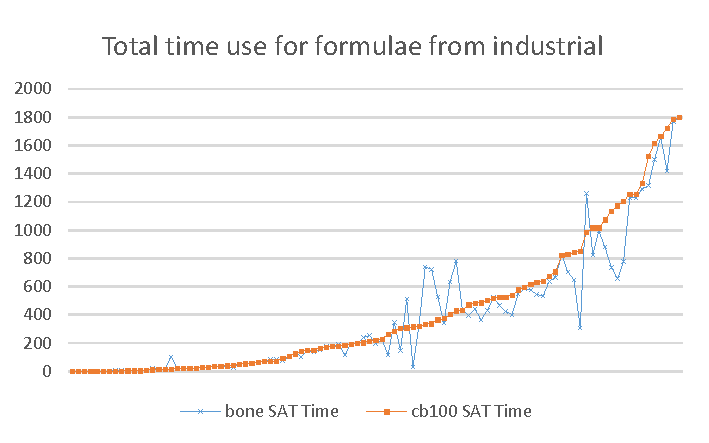
\includegraphics[scale=0.8]{ind2.pdf}
   \caption{Experimental results on industrial formulae}
   \label{fig:ind-time}
\end{figure}

\subsection{Experimental Results on Random Formulae}
In this section, we present experimental results on random formulae. Before presenting the overview of the experiments of the whole random formulae, we tested 100 random formulae from 6606 ones, which leads to finding what kind of formula are suitable to be solved by \tool.

\begin{figure}
    \centering
    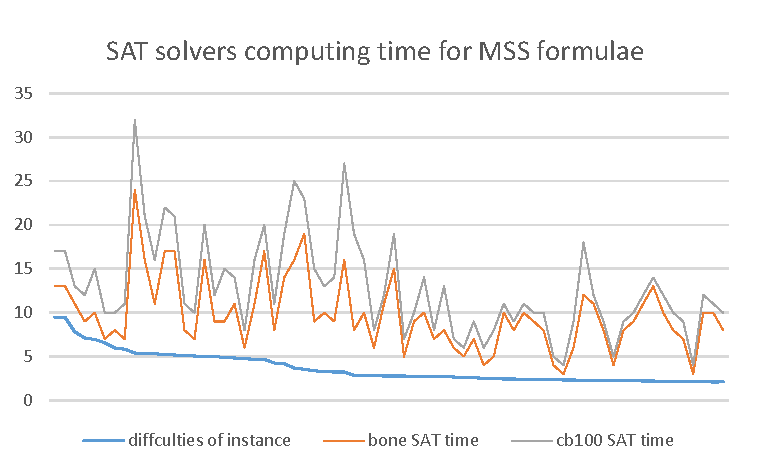
\includegraphics[scale=0.7]{mcs.pdf}
   \caption{Overview of results on industrial formulae}
   \label{fig:mcs-time}
\end{figure}

\begin{figure}[t]
\centering
\subfloat[cb100 performs better]{

\centering
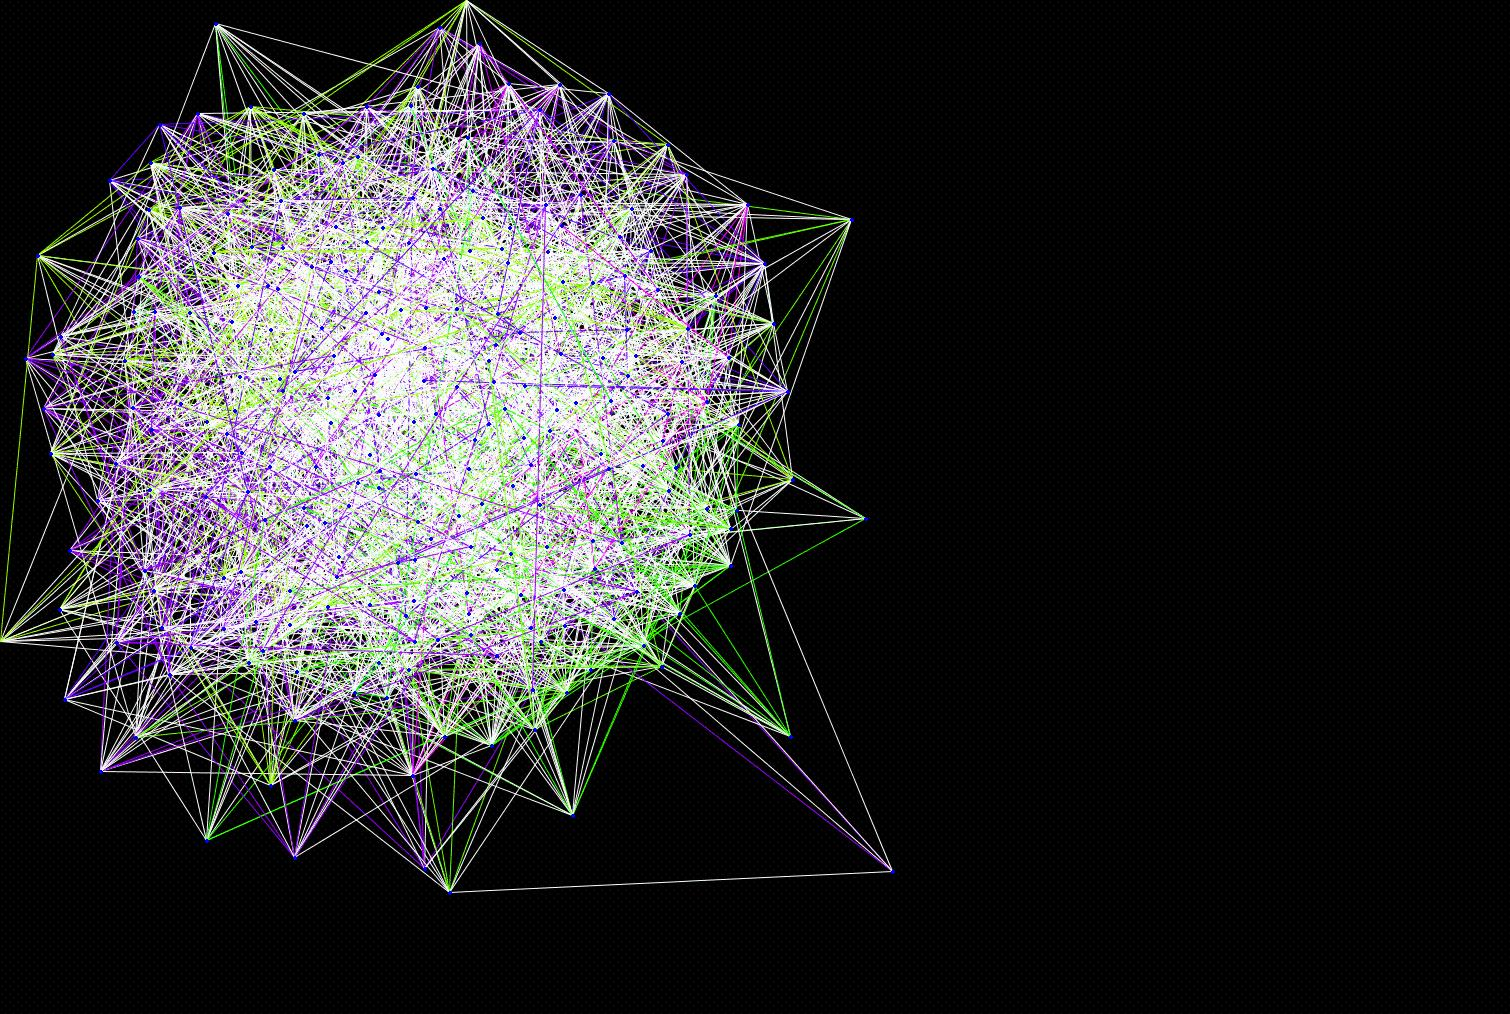
\includegraphics[width=.5\linewidth-0.45mm]{cb100.jpg}
}
\subfloat[\tool performs better]{
\centering
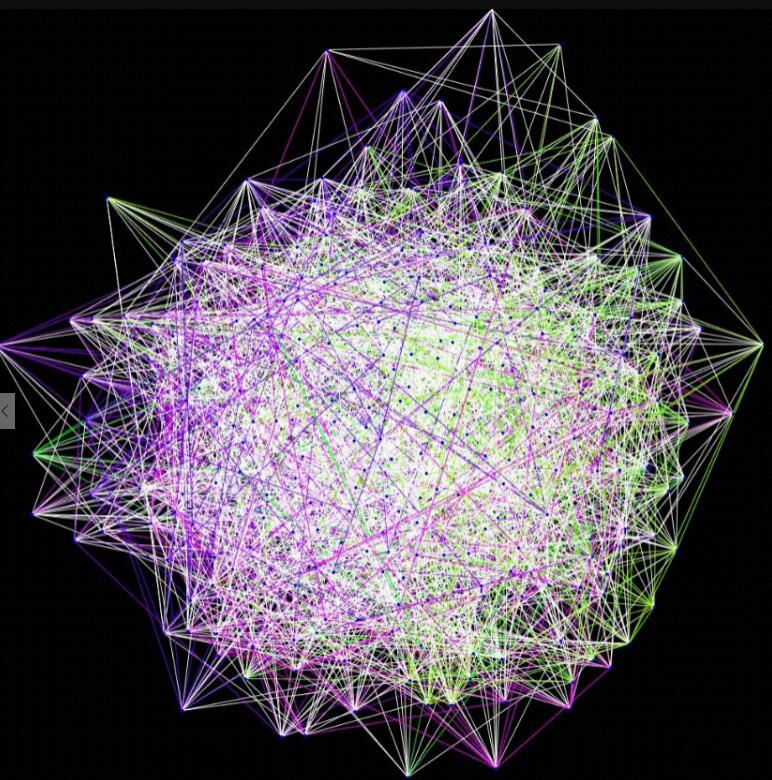
\includegraphics[width=.5\linewidth-0.45mm]{bone.jpg}
}
\caption{Community structures}
\label{fig:cs}
\end{figure}

\begin{table*}[!htb]
\begin{tabular}{c|c|c|c|c|c|c|c|c}
\hline
\multirow{2}{*}{} & \multicolumn{2}{c|}{Simple} & \multicolumn{2}{c|}{Medium} & \multicolumn{2}{c}{Hard}& \multicolumn{2}{|c}{Total} \\
\cline{2-9}
  & SAT Time (s) & SAT Calls & SAT Time (s)& SAT Calls & SAT Time (s)& SAT Calls&SAT Time (s)& SAT Calls \\
\hline
\tool& 6874.5   & 85570 & 35853   & 1332334 & 3577.9   & 76449  & 50183.02   & 1508723 \\ \hline
cb100 & 4413.5   & 86232 & 39040   & 1353258 & 5893.4   & 78114& 50414.04   & 1532372  \\
\hline
\end{tabular}
\caption{Results of random formulae}
\label{tab:mcs-graph}
\end{table*}
Figure \ref{fig:mcs-time} depicts the running time of results on  randomly formulae.
%selected 100 random formulae out of 6606 whose time of computing the first model range from 0s to more than 4s.
This result demonstrates that there is no correlation between the running time of backbone computing and running time of computing the first model, which is different from the result on industrial formulae. The reason is that random formulae have more complex community structures \cite{NZG2014,LJG2015SAT,LJG015}. Therefore, we cannot use running time of computing the first model to measure how hard a formula is.
To measure hardness of random formulae, we investigated community structures of all the random formulae, as it is already known that community structure of a formula affects the performance of conflict-driven clause learning based SAT solvers \cite{NZG2014}.


We constructed the community structures of all the random formulae using use SATGraph \cite{NZW2015}.
We observed that \textit{cb100} performs better on formulae whose community structures are divergent, i.e., there are vertexes far from the center of structures.
Figure \ref{fig:cs}(a) shows the community structure of one formula on which \textit{cb100} performs better.
While \tool performs better on formulae whose community structures are focusing.
Figure \ref{fig:cs}(b) shows the community structure of one formula on which \tool performs better.



Based on this observation, we divide 6606 random formulae into three groups according to their community structures.
The \emph{simple group} contains 371 formulae whose community structures are divergent,
the \emph{hard group} contains 337 formulae whose community structures are focusing,
and the \emph{medium} group contains 5898 formulae between divergent and focusing.


Table \ref{tab:mcs-graph} shows the experiments results on these three groups. \textit{cb100} performs better than \tool on the simple group, as \textit{cb100} tries to find a backbone literal by complementing models as soon as possible, which are the vertexes far from the center.
\tool outperforms \textit{cb100} for both medium group and hard group.
\tool reduces by 8\% for medium group and by 40\% for hard group of the total running time.


%\begin{figure}
%    \centering
%    \includegraphics[scale=0.2]{\textit{cb100}.jpg}
%   \caption{Community Structure of Formula Performs better with \textit{cb100}}
%   \label{fig:\textit{cb100}}
%\end{figure}

%\begin{figure}
%    \centering
%    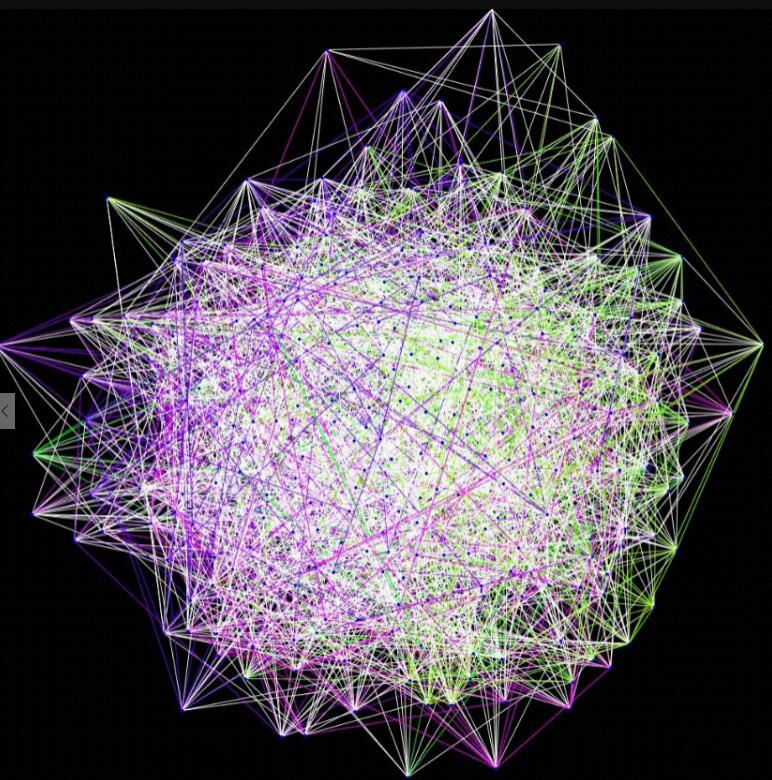
\includegraphics[scale=0.2]{bone.jpg}
%   \caption{Community Structure of Formula Performs better with \tool}
%   \label{fig:bone}
%\end{figure}


The experimental results show that \tool performs better than \textit{cb100} on hard random formulae and is comparable to \textit{cb100} on simple formulae.




